\documentclass[a4paper,12pt]{article}

% Paquetes básicos
\usepackage[utf8]{inputenc}
\usepackage[T1]{fontenc}
\usepackage[spanish]{babel}
\usepackage{graphicx}
\usepackage{xcolor}
\usepackage{lipsum}
\usepackage{geometry}
\geometry{top=3cm, bottom=3cm, left=2.5cm, right=2.5cm}
\usepackage{pdfpages}

% Paquetes para diseño
\usepackage{titlesec}
\usepackage{fancyhdr}
\usepackage{amsmath}
\usepackage{amssymb}
\usepackage{hyperref}

% Paquetes para el entorno lstlisting
\usepackage{listings}
\usepackage{inconsolata}

% Paquete para fondo
\usepackage{background}

% Configuración de lstlisting
\lstset{
    language=Python,
    basicstyle=\ttfamily\small,
    keywordstyle=\color{blue}\bfseries,
    stringstyle=\color{teal},
    commentstyle=\color{gray}\itshape,
    numbers=left,
    numberstyle=\tiny\color{gray},
    backgroundcolor=\color{black!5},
    frame=single,
    rulecolor=\color{black!50},
    breaklines=true,
    captionpos=b,
    showstringspaces=false
}

% Configuración de título
\titleformat{\section}{\normalfont\Large\bfseries}{\thesection}{1em}{}

% Información del documento
\title{
    \vspace{-2cm}
    
\includegraphics[width=0.3\textwidth]{images/etsiit.png} \\ % Cambia el logo si es necesario
    \LARGE Ingeniería Informática + ADE\\
    \large Universidad de Granada (UGR)\\[1cm]
}
\author{\textbf{Autor:} Ismael Sallami Moreno}
\date{\textbf{Asignatura:} Sistemas Concurrentes y Distribuidos}

% Configuración del fondo
\backgroundsetup{
    scale=1,
    color=black,
    opacity=0.2,
    angle=0,
    position=current page.south,
    vshift=0pt,
    hshift=0pt,
    contents={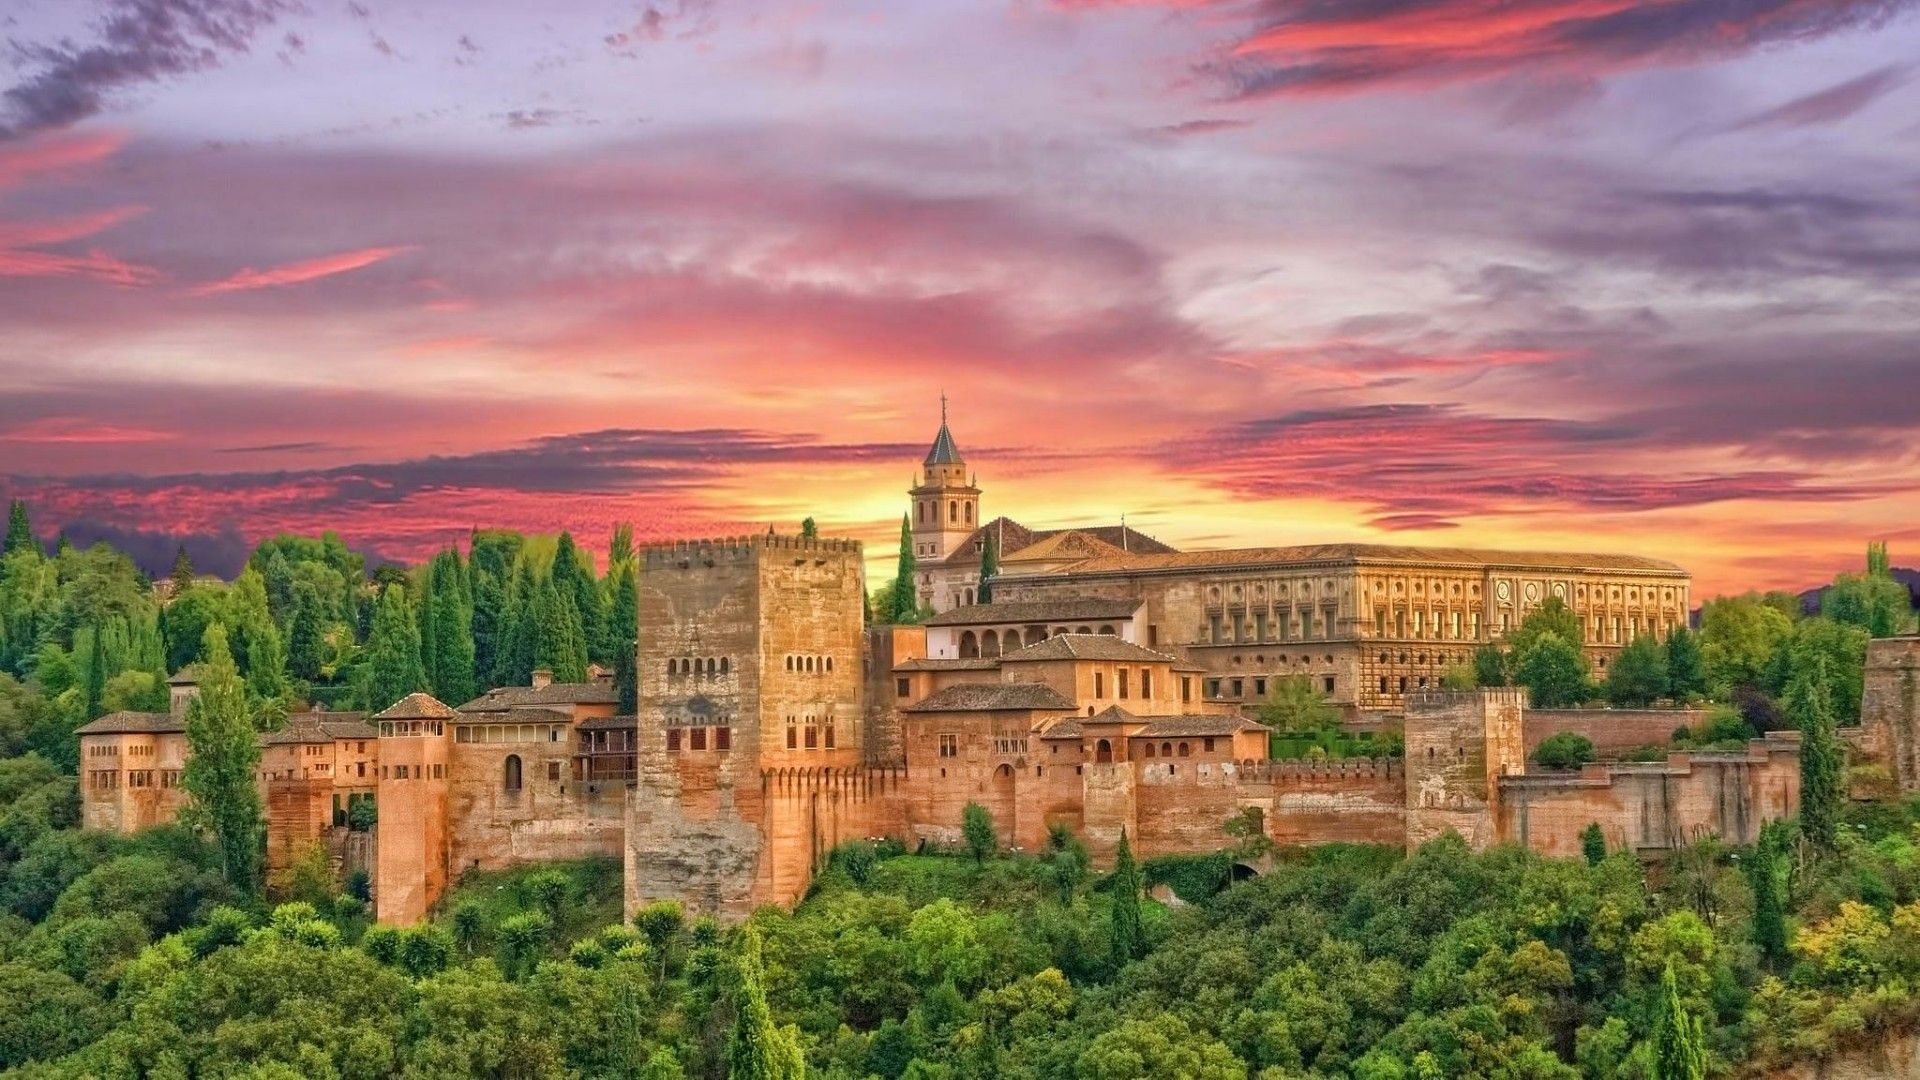
\includegraphics[width=\paperwidth,height=\paperheight,keepaspectratio]{images/granada.jpg}}
}

% Inicio del documento
\begin{document}

% Portada
\maketitle
\thispagestyle{empty}

\begin{center}
    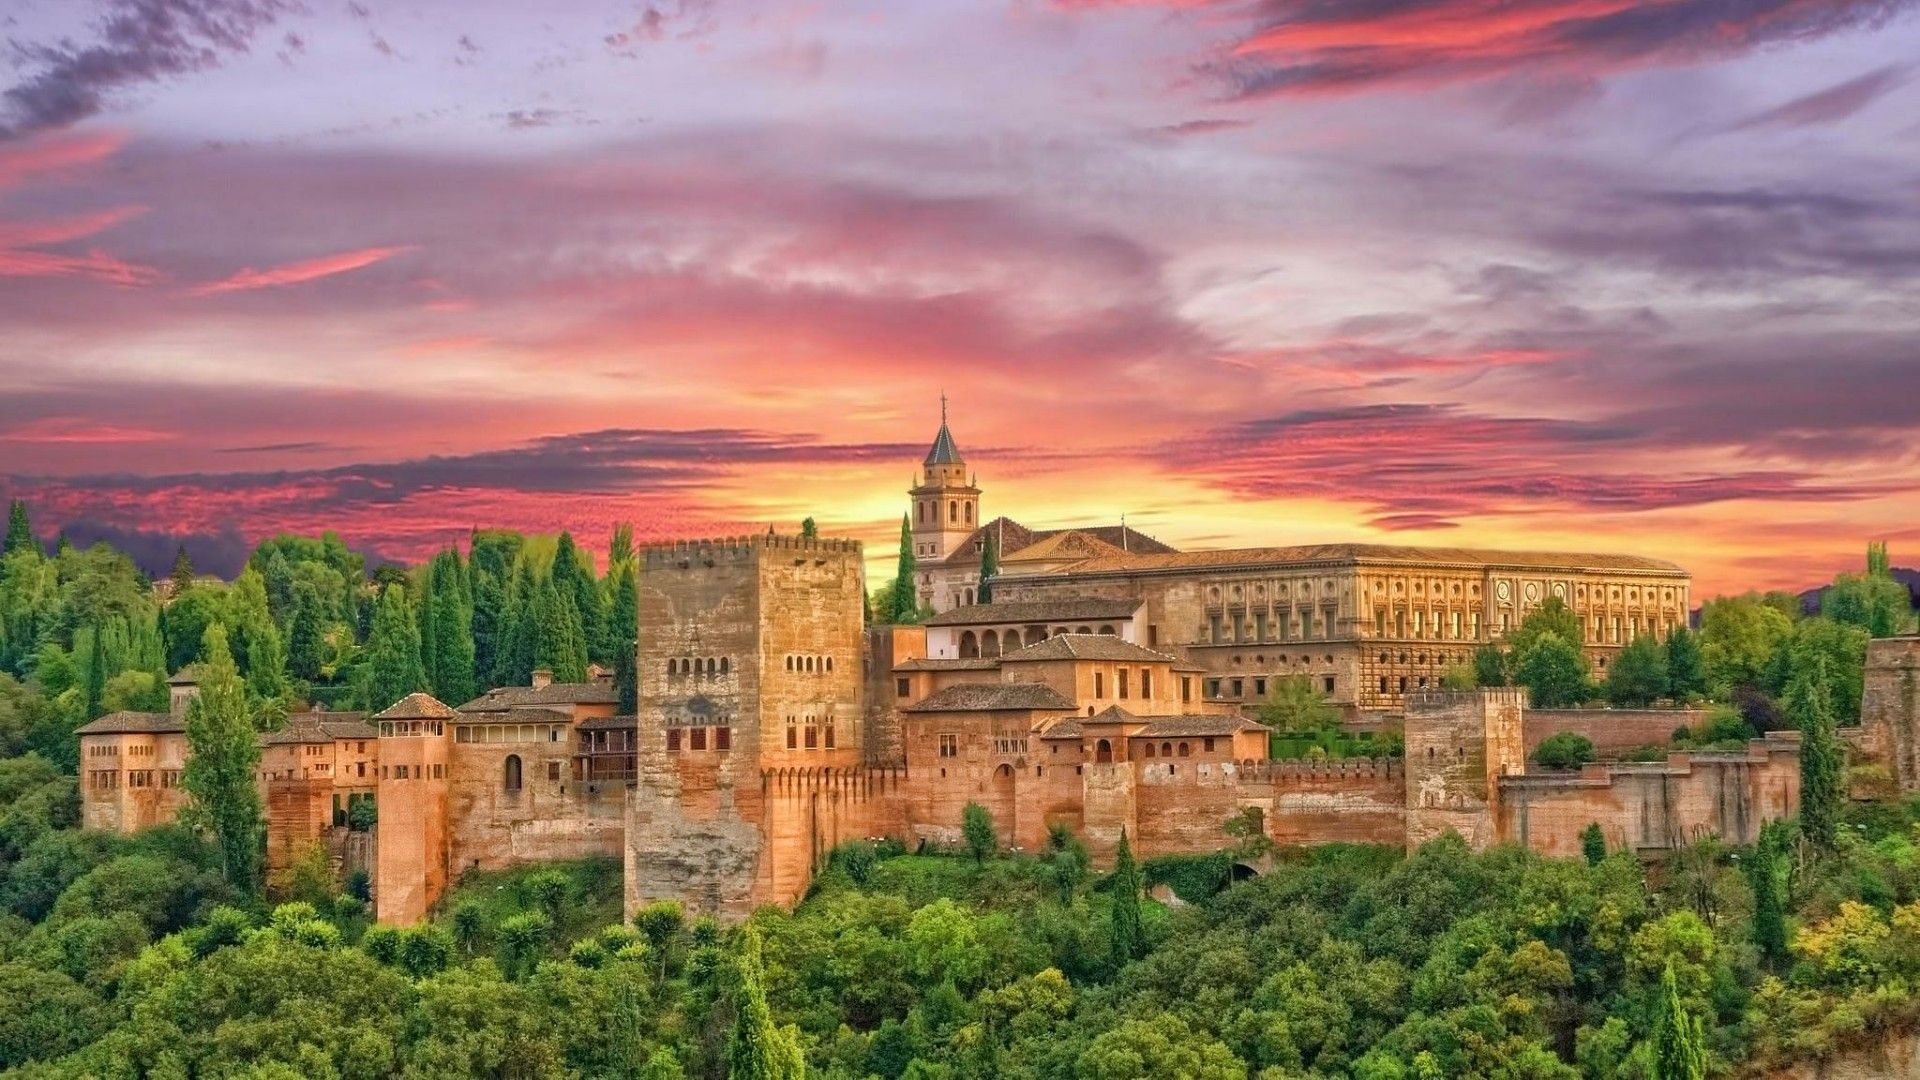
\includegraphics[width=\textwidth,height=0.4\textheight,keepaspectratio]{images/granada.jpg} \\ % Añade tu imagen de fondo
    \vfill
\end{center}

\newpage

% Índice (opcional)
\tableofcontents
\newpage

\section{Teoria}
\subsection{Tema 1}

\includepdf[pages=-]{../Tema1/T1.pdf}
\subsection{Tema 2}
\subsection{Tema 2.1}

\includepdf[pages=-]{../Tema2/T2-1.pdf}
\subsection{Tema 2.2}

\includepdf[pages=-]{../Tema2/T2-2.pdf}
\subsection{Mapa de Ideas Tema 1 y 2}
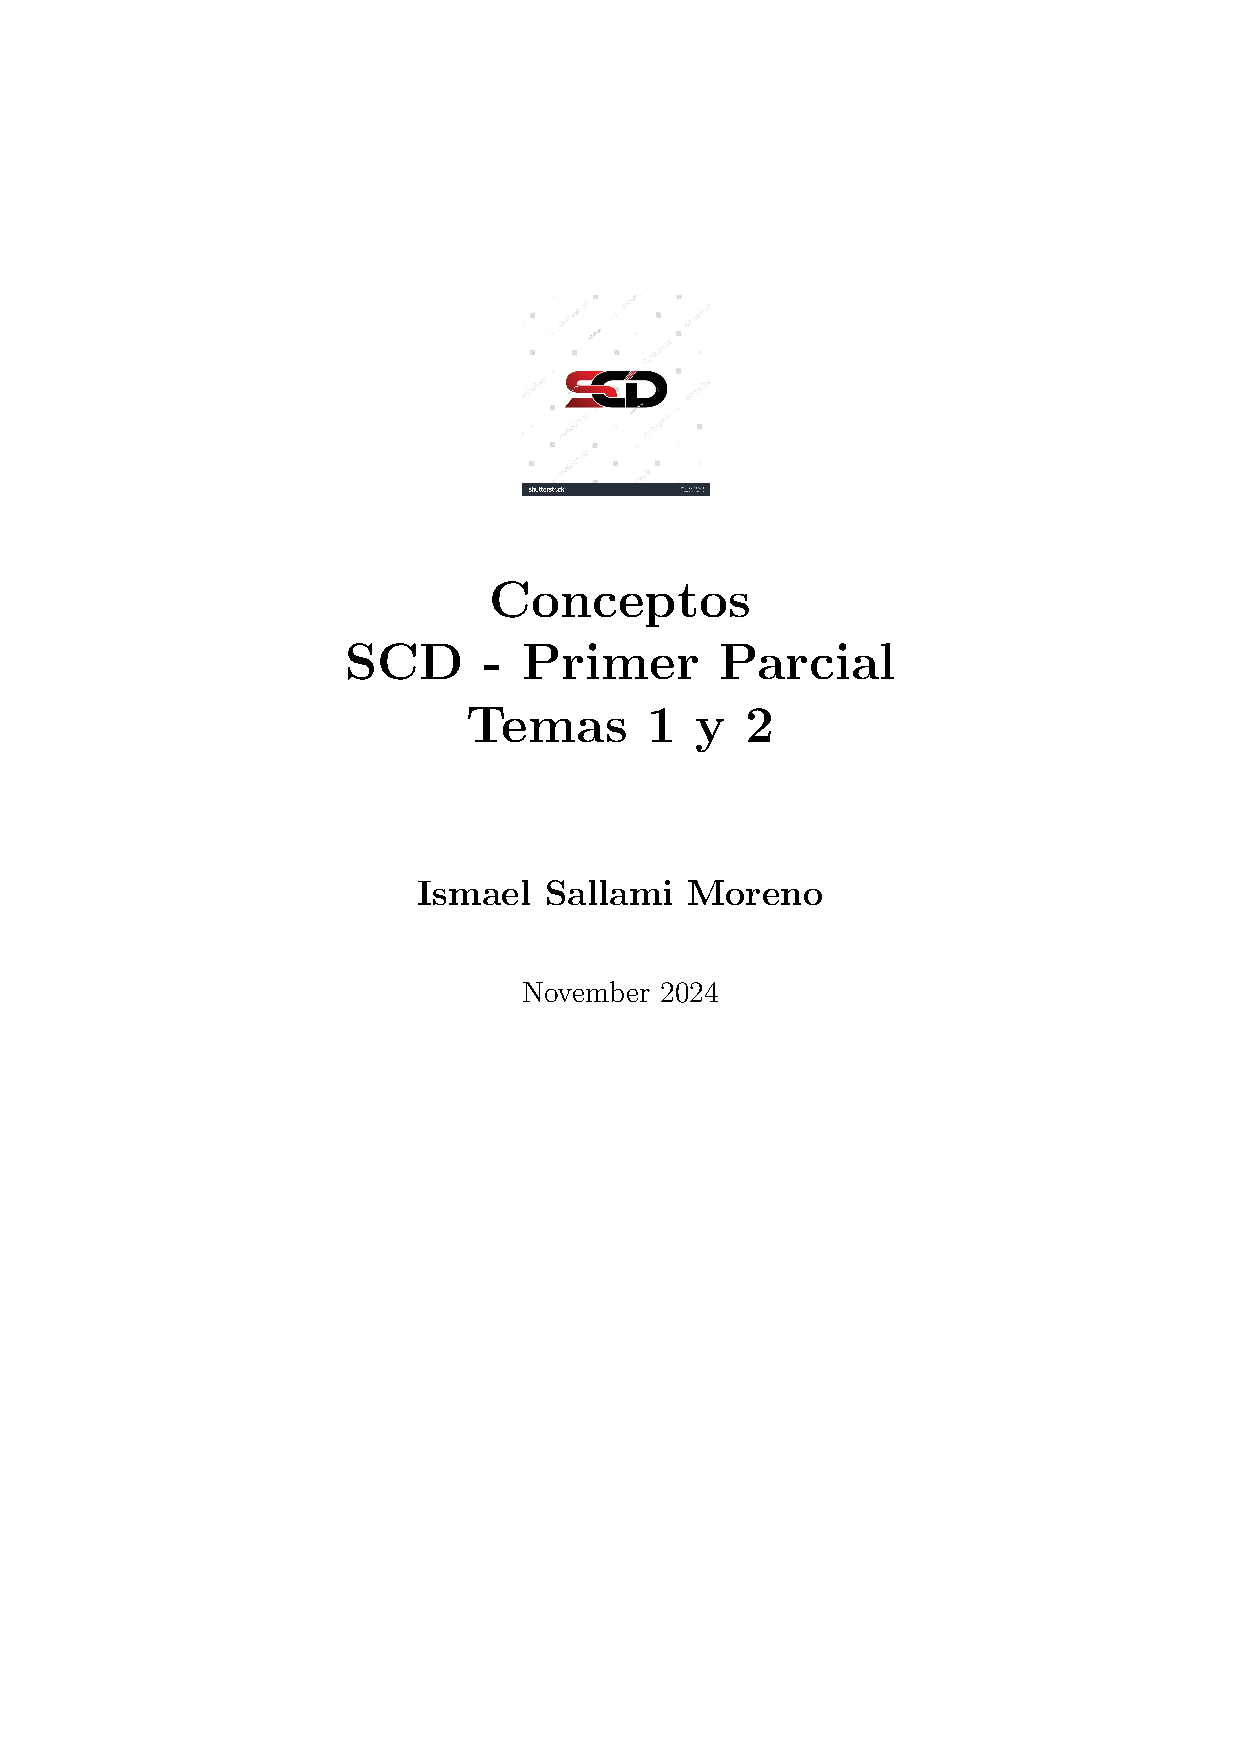
\includepdf[pages=-]{../Tema2/Mapa1y2.pdf}
\subsection{Tema 3}
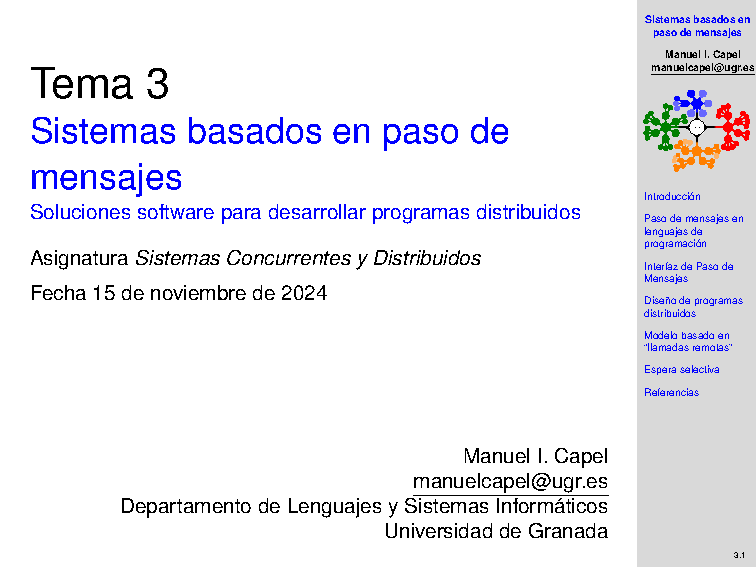
\includepdf[pages=-]{../Tema3/T3.pdf}
\subsection{Tema 4}
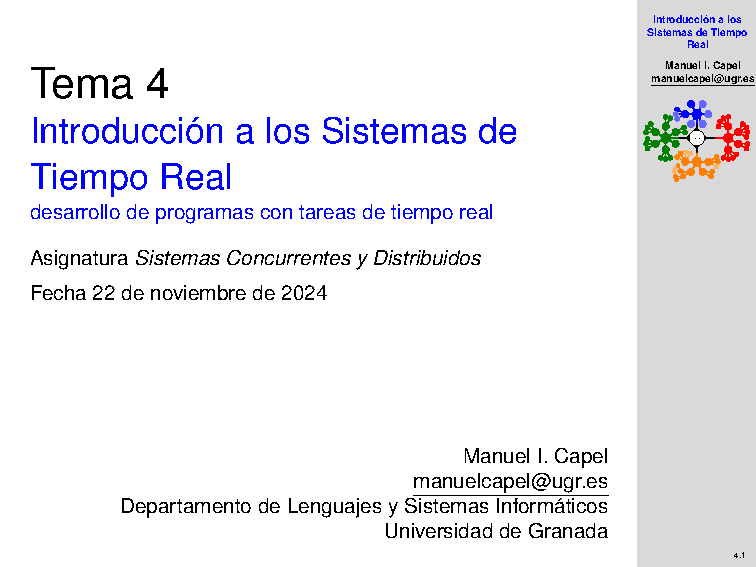
\includepdf[pages=-]{../Tema4/T4.pdf}

\section{Resúmenes}
\includepdf[pages=2-]{../../Resumenes/ETSIIT/build/Apuntes.pdf}



\section{Relaciones de Ejercicios}
\subsection{Relación 1}
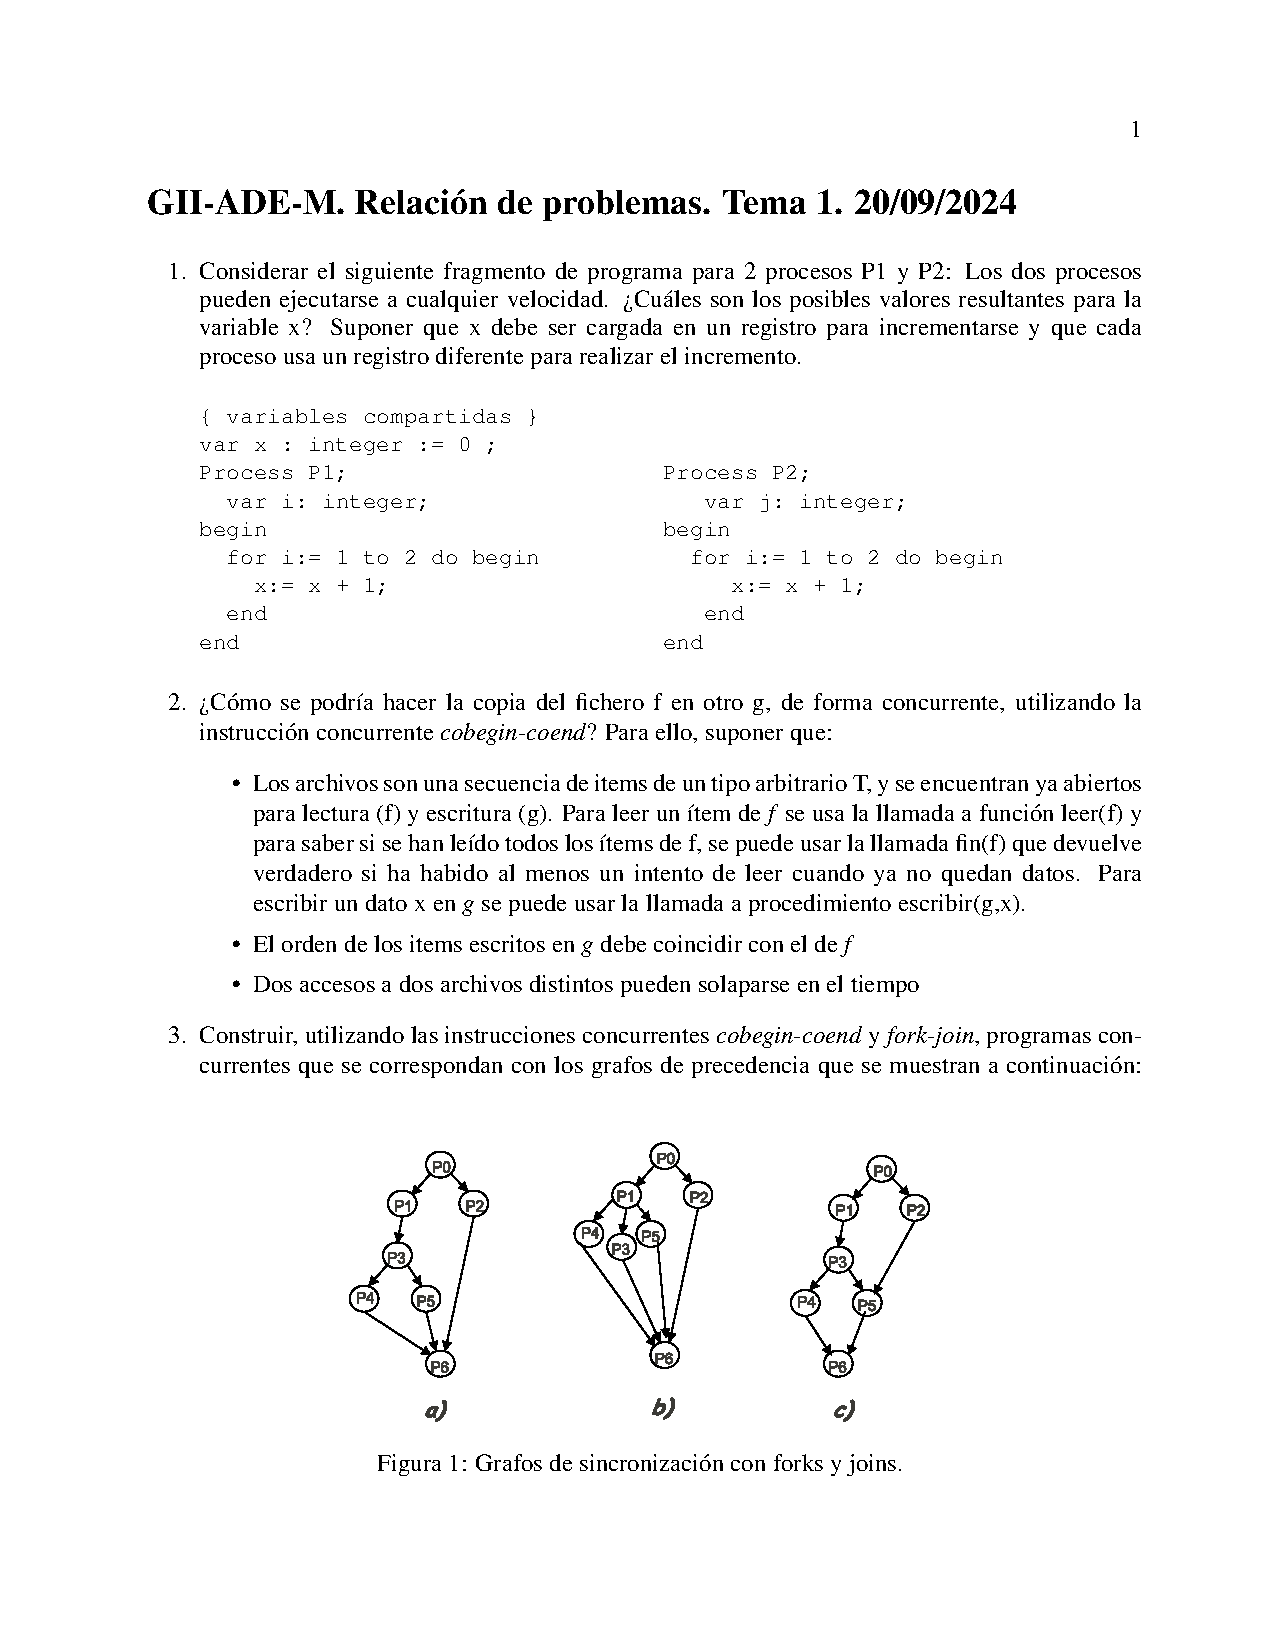
\includepdf[pages=-]{../Tema1/EnunciadosT1.pdf}
\subsubsection{Solución}
La Solución la puedes encontrar:
\begin{itemize}
    \item \href{https://github.com/ElblogdeIsmael/ElblogdeIsmael.github.io/tree/main/Asignaturas/Tercer%20A%C3%B1o/SCD/Teoria/Tema1/RelacionEjerciciosTema1.md}{Relación de Ejercicios Tema 1 en markdown}
    \item \href{https://github.com/ElblogdeIsmael/ElblogdeIsmael.github.io/tree/main/Asignaturas/Tercer%20A%C3%B1o/SCD/Teoria/Tema1/RelacionEjerciciosTema1.pdf}{Relación de Ejercicios Tema 1 en pdf}
\end{itemize}

\subsection{Relación 2}
\subsubsection{Relaciones 2.1}

\subsubsection{Solución}
La Solución la puedes encontrar:
\begin{itemize}
    \item \href{https://github.com/ElblogdeIsmael/ElblogdeIsmael.github.io/tree/main/Asignaturas/Tercer%20A%C3%B1o/SCD/Teoria/Tema2/RelacionEjerciciosTema2.md}{Relación de Ejercicios Tema 1 en markdown}
\end{itemize}
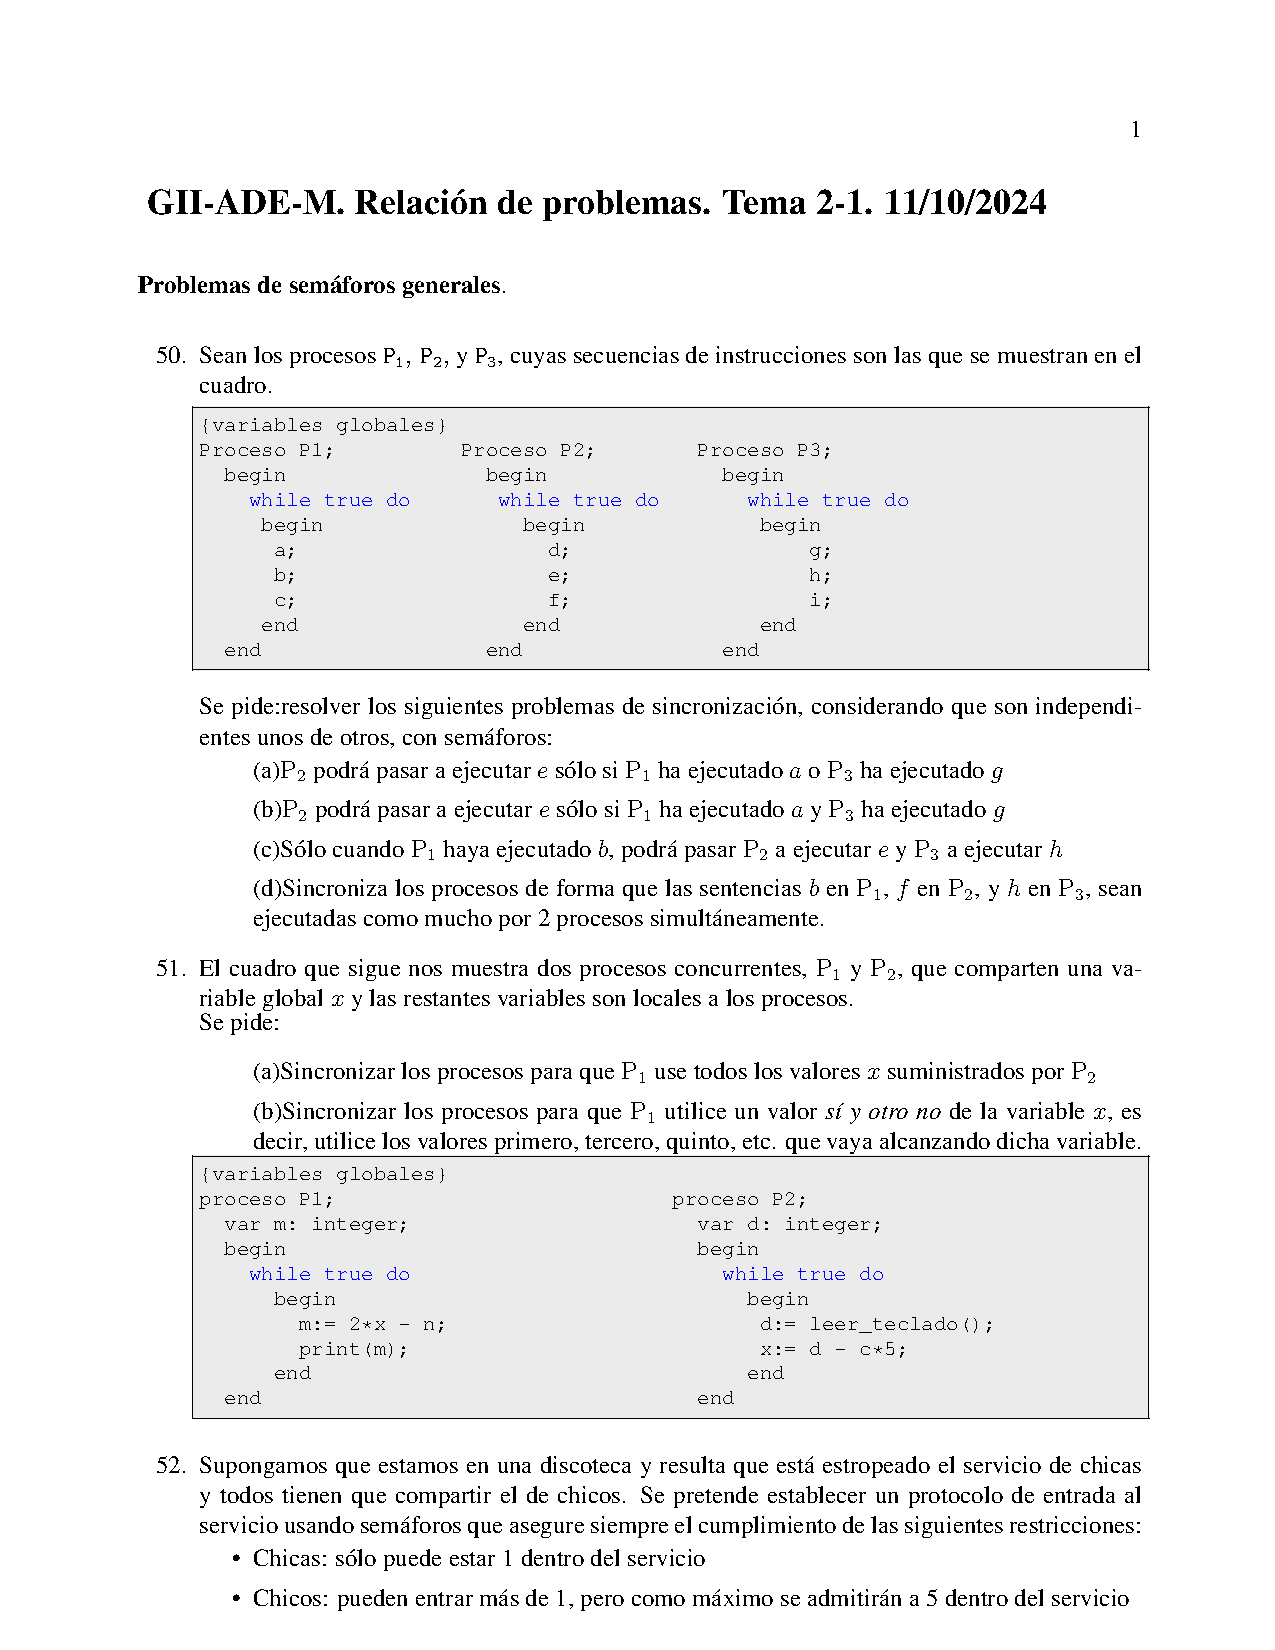
\includepdf[pages=-]{../Tema2/EjerciciosT2-1.pdf}
\subsubsection{Relaciones 2.2}
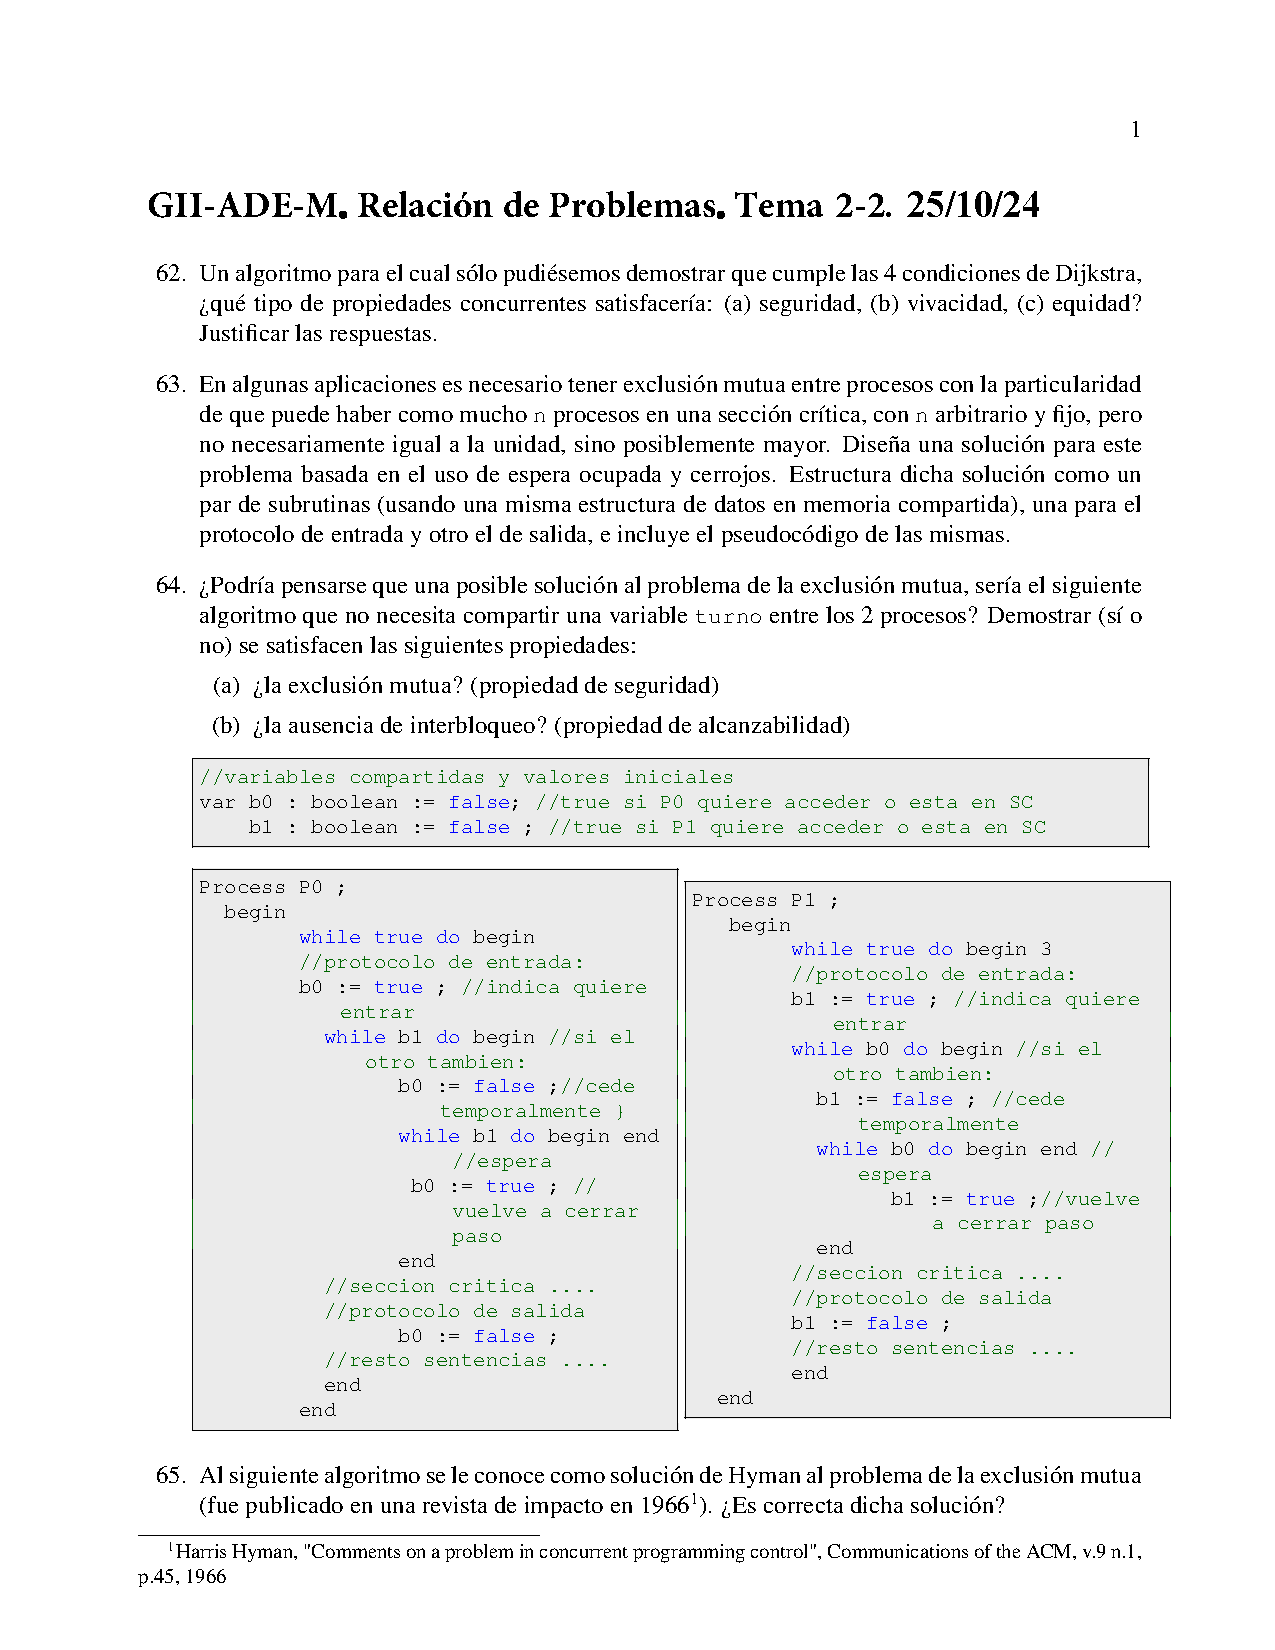
\includepdf[pages=-]{../Tema2/EjerciciosT2-2.pdf}

\subsection{Relacion 3}
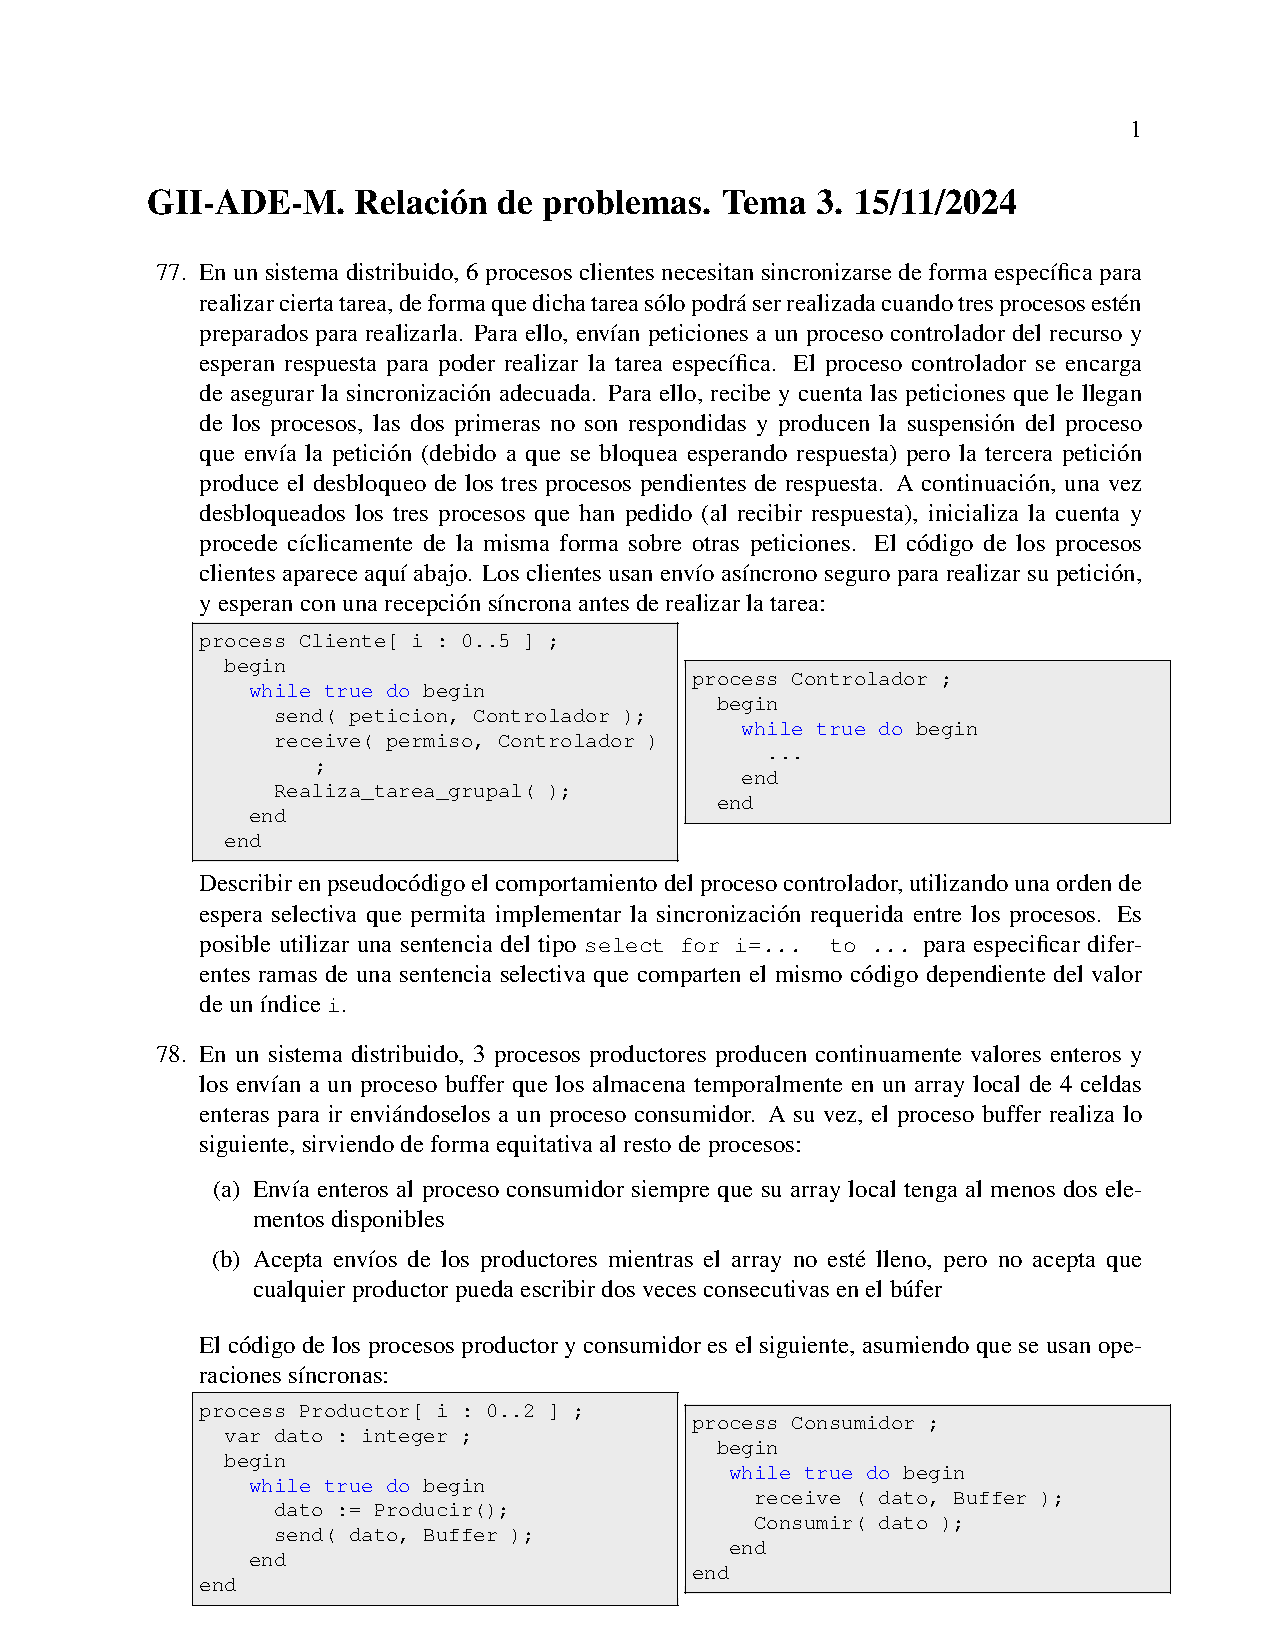
\includepdf[pages=-]{../Tema3/EjerciciosT3.pdf}
\subsubsection{Solución}
\includepdf[pages=3-]{../Tema3/SolucionesEjercicios/ETSIIT/build/Ejerciciost3.pdf}





\subsection{Relacion 4}
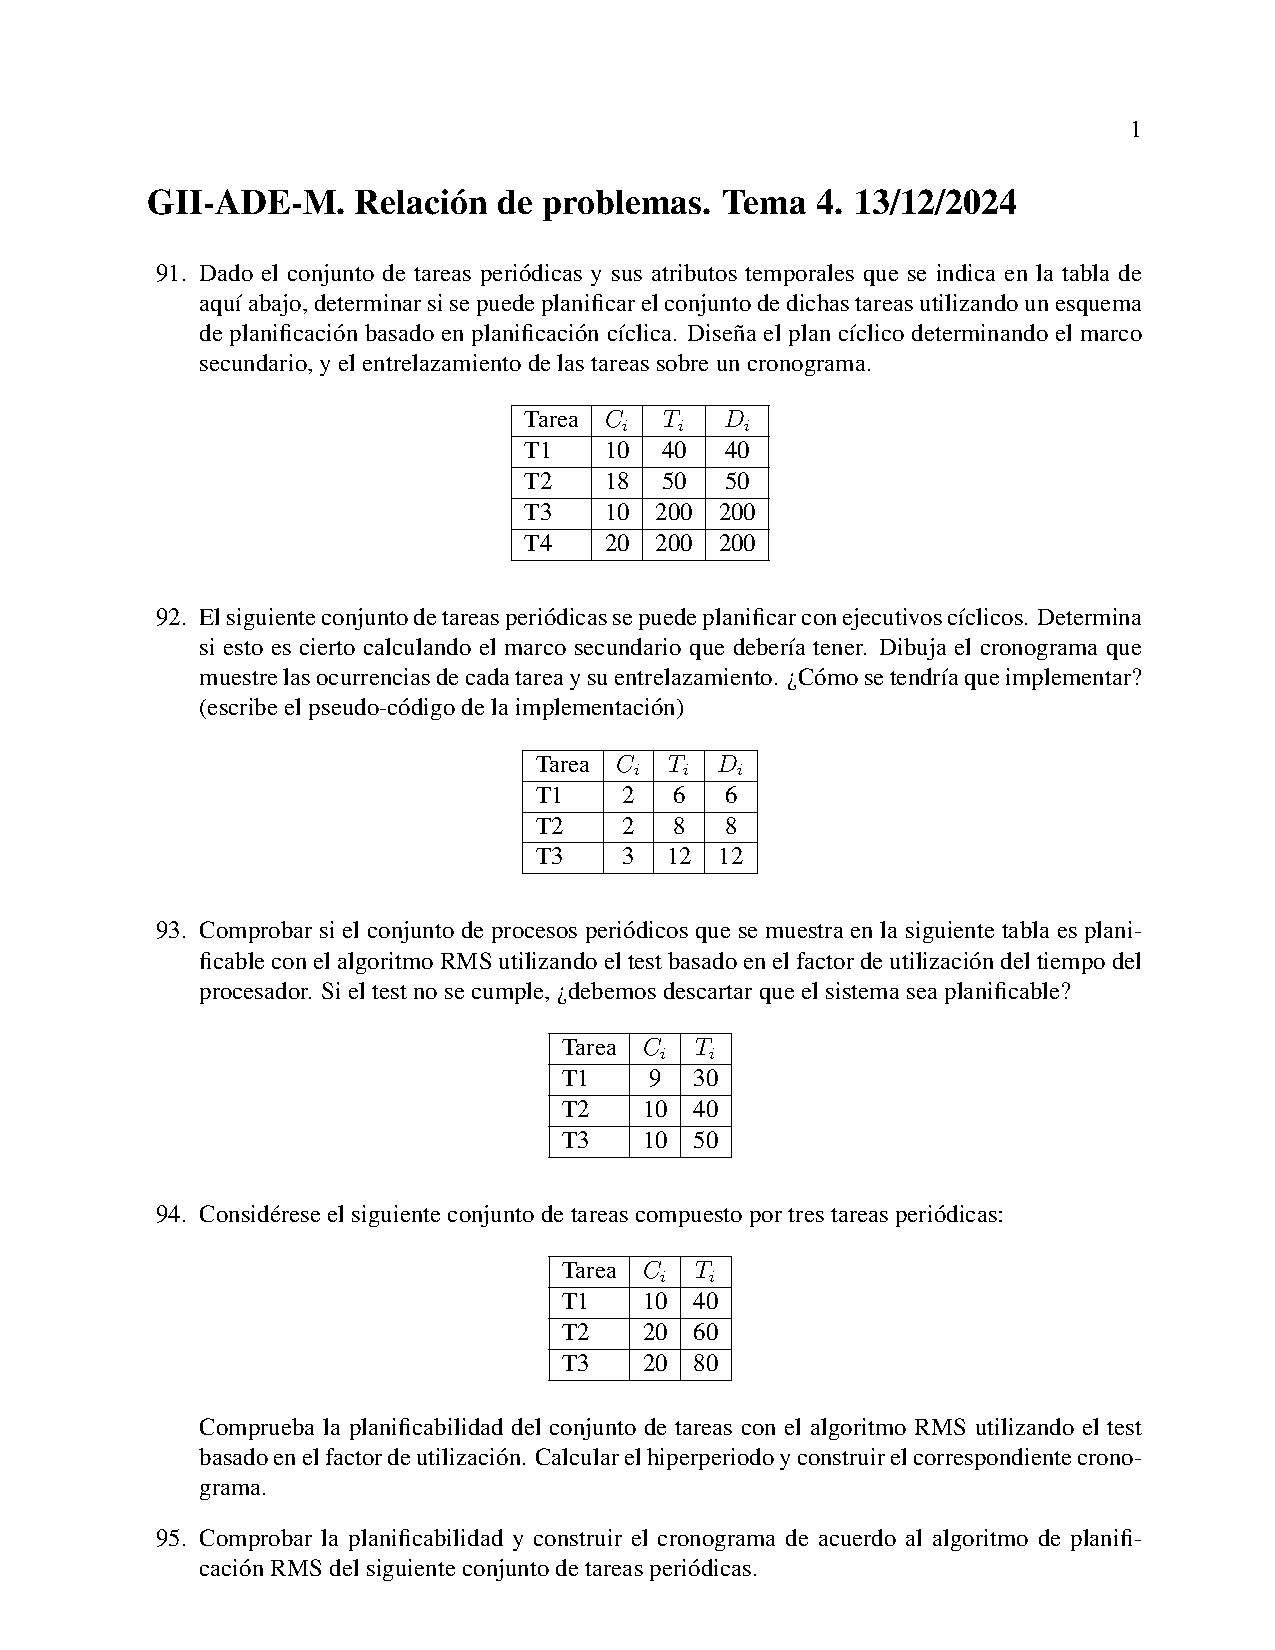
\includepdf[pages=-]{../Tema4/EjerciciosT4.pdf}

\section{Actividades Extras}
\subsection{Criba de Eratóstenes}
%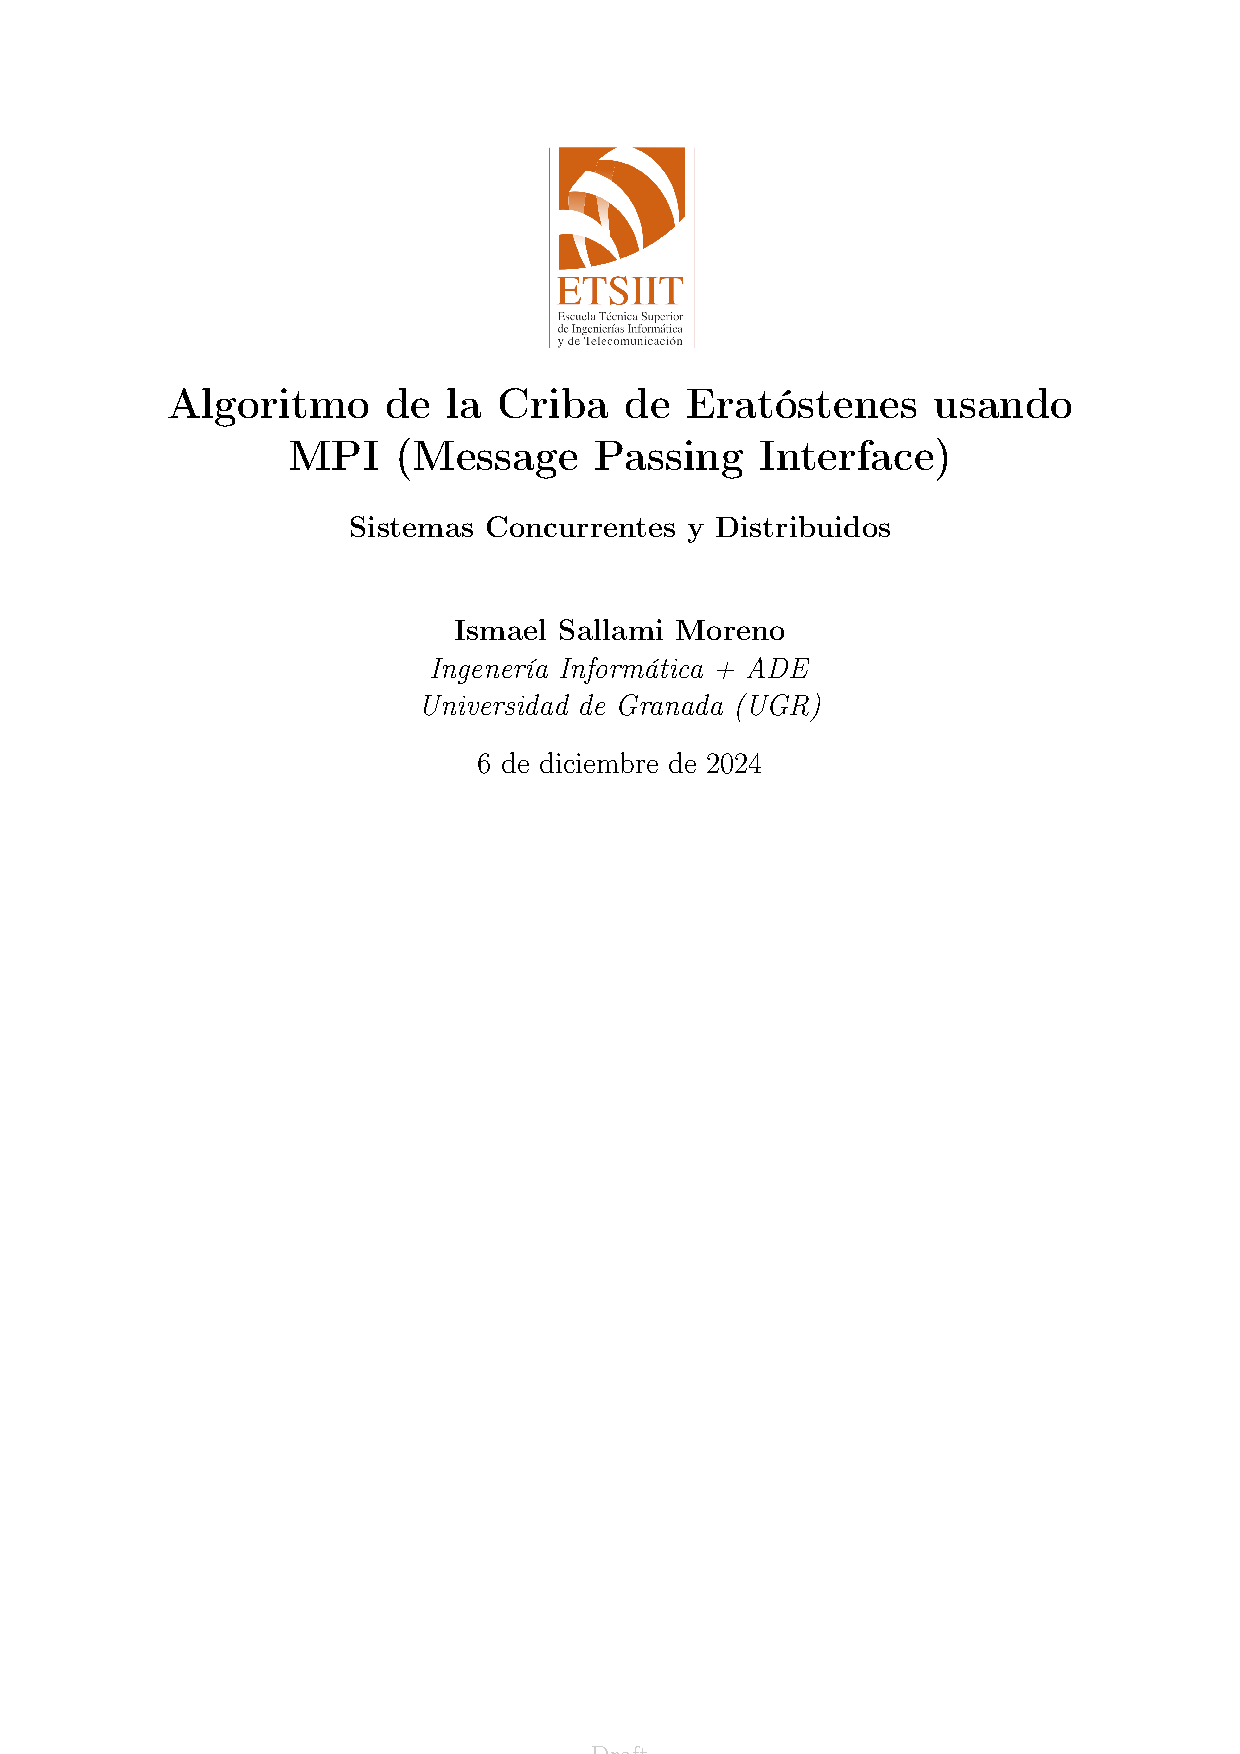
\includepdf[pages=-]{../Actividad_Extra/cribadeErastotenes/ETSIIT/build/Erastotenes.pdf}
Para ver el archivo pdf pinche 
\href{https://github.com/ElblogdeIsmael/ElblogdeIsmael.github.io/blob/main/Asignaturas/Tercer%20A%C3%B1o/SCD/Teoria/Actividad_Extra/cribadeErastotenes/ETSIIT/build/Erastotenes.pdf}{aquí.}

\subsection{Demostración de las Propiedades de un Algoritmo de Exclusión Mutua}
Para ver el archivo pdf pinche 
\href{https://github.com/ElblogdeIsmael/ElblogdeIsmael.github.io/blob/main/Asignaturas/Tercer%20A%C3%B1o/SCD/Teoria/Actividad_Extra/Demostracion_Prop_ALG_EM/ETSIIT/build/Demostracion.pdf}{aquí.}

\newpage

\section{Referencias}
\begin{itemize}
    \item Diapositivas de clase.
\end{itemize}






\end{document}
